\documentclass[12pt,a4 paper]{book}
\usepackage[utf8]{inputenc}
\usepackage[english,russian]{babel}
\usepackage{misccorr}
\usepackage{graphicx}
\usepackage{amsmath}
\usepackage{mathtext}
\textwidth=17.2cm
\textheight=25cm
\oddsidemargin=--6mm
\evensidemargin=--6mm
\topmargin=--1mm

\usepackage{mathtools}
\usepackage{setspace}
\usepackage{amsfonts}
\usepackage[T2A]{fontenc}

\usepackage{graphicx}
\graphicspath{{pictures/}}
\DeclareGraphicsExtensions{.pdf,.png,.jpg}

\begin{document}
\begin{titlepage}
\begin{center}
\normalsize
МИНИСТЕРСТВО ОБРАЗОВАНИЯ И НАУКИ \\РОССИЙСКОЙ ФЕДЕРАЦИИ
\vspace{0.25cm}

МОСКОВСКИЙ ГОСУДАРСТВЕННЫЙ УНИВЕРСИТЕТ\\ им М.В.Ломоносова
\vspace{0.25cm}

Механико-математический факультет

Кафедра теории вероятностей
\vfill

\vfill

\textsc{\textbf{Курсовая работа}}\\[3mm]

{ “Обоснование на первый взгляд неожиданного свойства образов допустимых портфелей. Расчеты реального примера.”  }
\bigskip

\end{center}
\vfill

\newlength{\ML}
\settowidth{\ML}{«\underline{\hspace{0.7cm}}» \underline{\hspace{2cm}}}
\hfill\begin{minipage}{0.4\textwidth}
\textbf{Выполнил:}\\ студент 4 курса 431 группы\\ Ковальчук А.А.

\end{minipage}%
\bigskip

\hfill\begin{minipage}{0.4\textwidth}
\textbf{Научный руководитель:}\\ доц. кафедры теории веротностей\\ Жуленёв С.В.
\end{minipage}%
\vfill

\begin{center}
\vfill

\vfill
Москва, 2021 г.
\end{center}
\end{titlepage}

\thispagestyle{empty}

\smallskip
\begin{center}
{\bf\Large Содержание}
\end{center}
\begin{enumerate}
\item[1] \textbf{Введение} 

\item[2] \textbf{Точка внутри пули Марковица имеет два прообраза}
\begin{enumerate}
\item[2.1.] Постановка задачи
\item[2.2.] Решение
\end{enumerate}
\item[3] \textbf{Найти второй прообраз у конкретной точки}
\begin{enumerate}
\item[3.1.] Постановка задачи
\item[3.2.] Решение
\end{enumerate}
\item[4] \textbf{О двух прообразах эффективной границы в модели Марковица}
\begin{enumerate}
\item[4.1.] Постановка задачи
\item[4.2.] Решение
\end{enumerate}
\item[5] \textbf{Список используемой литературы}
\end{enumerate}

\newpage
\section*{1. Введение}
\smallskip
Цель данной курсовой работы состоит в том, чтобы ознакомить читателя со свойствами образов допустимых портфелей. Используя теорию из главы 1, будет показано, что любая точка внутри пули Марковица имеет два прообраза (один из которых очевиден). Дополнительно будет вычислен прообраз конкретной точки, параметры которой заданы в примере главы 1. После чего, опираясь на решения и теорию, будут найдены два прообраза эффективной границы в модели Марковица.

\newpage
\section*{2. Точка внутри пули Марковица имеет два прообраза}
\smallskip
\begin{enumerate}
\item[2.1.] \textbf{Постановка задачи}

Пусть о всех 3-x активах портфеля известны вектор ожидаемой доходности $m$ и матрица ковариаций $\Sigma$, причем $0 < m_1 < m_2 < m_3$, а $|\Sigma| \neq 0$. В этом случае внутренняя точка пули Марковица имеет два прообраза на плоскости $(x_2,x_3)$ или в пространстве $(x_1,x_2,x_3)$, лежащие по разные стороны от прообраза кривой минимального риска.

\item[2.2.] \textbf{Решение}
\smallskip

Рассмотрим помимо данной точки $(\sigma, \mu)$ внутри пули точку $(\sigma_\mu, \mu)$, лежащую на ее границе, т.е. на кривой минимального риска. Как известно, этой второй точке соответствует единственный вектор $x$, принадлежащий прообразу кривой минимального риска в $R^3$, а прообразы $x + y$ исходной точки задаются с помощью вектора $y=y(x)$ следующим образом:

\begin{equation}
min(x^T \Sigma x)\equiv \sigma_\mu^2,  \quad e^T x = 1, \quad m^t x = \mu, 
\label{eq:ref}
\end{equation}

\begin{equation}
\mu^2 = (x+y)^T \Sigma (x+y), \quad e^t y = 0 , \quad m^T y = 0.
\label{eq:ref}
\end{equation}

Из теоремы 2 имеем, что решение экстремальной задачи $(1)$ записывается в виде $u=x+\mu v$ при некоторых фиксированных векторах $u$ и $v$. С другой стороны, система двух уравнений из $(2)$ относительно 3-x переменных $y_i$ позволяет выразить вектор $y$ через его третью компоненту следующим образом:

\begin{center}
$y=y_3 z$, \quad $z=(\frac{m_3-m_2}{m_2-m_1}, \frac{m_1-m_3}{m_2-m_1},   1)$.
\end{center}
Поэтому первое равенство в $(2)$ можно переписать в виде:
\begin{equation}
d\equiv \sigma - \sigma_\mu^2 = 2 y^T \Sigma (u+\mu v)+ y^T\Sigma y \Leftrightarrow a y_3^2+2(b+\mu c)y_3-d=0,
\label{eq:ref}
\end{equation}

где $a=z^T\Sigma z$, $b=z^T\Sigma u$,  $c=z^T\Sigma v$. Отсюда имеем, что: 
\begin{center}
$y_3=\frac{-(b+\mu c) \pm \sqrt{(b+\mu c)^2+ad}}{a}$
\end{center}

Значит, независимо от знака суммы $b+\mu c$ оба корня $(y_3)_{1,2}$ уравнения (3) имеют разные знаки. Это следует из того, что  $a>0$, $d>0$ в силу предположений и того, что вектор $z$ ненулевой.

Итак, у каждой внутренней точки пули два прообраза $x+(y_3)_{1,2} z$. Остается заметить, что оба прообраза лежат на прямой с направляющим вектором $z$ и проходящей через точку $x$, причем по разные стороны от $x$. Кроме того, ни один из них не может лежать на прямой -- прообразе минимального риска. В самом деле, оба вектора $x+y$ отличается от $x$, поэтому в предположении противного получим, что у отвечающих портфелям $x+y$ и $x$ активов должны быть разные ожидаемые доходности, а она у всех равна $\mu$.
\end{enumerate}

\newpage
\section*{3. Найти второй прообраз у конкретной точки}
\smallskip
\begin{enumerate}
\item[3.1.] \textbf{Постановка задачи}
Найти прообраз точки $(\sigma,\mu)=(0.25,0.2)$, отличной от точки $(x_1,x_2,x_3)=(0,0,1)$, используя пример 1 из п.3.4.
\item[3.2.] \textbf{Решение}
\smallskip
Для начала выпишем матрицу ковариаций и формулы, которые мы будем использовать для вычисления необходимых величин. Формулы выведены в соответствующем пункте главы 1 и предыдущем пункте: 

\begin{center}
\Sigma = \begin{pmatrix}
$0.0784 -0.067 0.0175$\\
$-0.067 0.0576 0.0120$\\
$0.0175 0.0120 0.0625$\
\end{pmatrix} $\\
\end{center}

\begin{center}
\begin{math}
v\equiv \sigma^2 = \alpha_2\mu^2+2\alpha_1\mu+\alpha_0, \end{math}
где  \alpha_0=u^T$\Sigma$$u$, \alpha_1=u^T$\Sigma$$v$, \alpha_2=v^T$\Sigma$$v$\\
\smallskip
$u$ $=$ {\gamma(m,m)\Sigma^{-1}e-\gamma(m,e)\Sigma^{-1}m}\over{R}$, $v$ $=$ {\gamma(e,e)\Sigma^{-1}m-\gamma(e,m)\Sigma^{-1}e}\over{R}$\\
\smallskip
$R$ $=$ \gamma(m,m)\gamma(e,e) - \gamma(e,m)\gamma(m,e) $>0$,
\gamma(y,z) $=$ $y^T\Sigma^{-1}z$ $=$$ $(y^T\Sigma^{-1},z)$, 
$x = u+\mu v$\\
\end{center}

Теперь, когда все формулы у нас перед глазами, произведем расчеты. Вычислять будем последовательно, чтобы ничего не пропустить:
\begin{center}
$\alpha_0 = 0.237$, $\alpha_1 = -1.4415$, $\alpha_2 = 9.843$ \\
$\sigma^2_{0.2} = 9.843*0.04-2.883*0.2+0.237 = 0.05412$ \\
$u = (1.578, 0.844, -1.422)$, $v = (-8.614, -2.770, 11.384)$
\end{center}
Теперь, зная $u$ и $v$, вычислим координаты вектора $x$ по формуле $x = u+\mu v$ и произведем дальнейшие расчеты:
\begin{center}
$x = (1.578-8.614\mu,0.844-2.77\mu,-1.422+11.384\mu) = (-0.1448, 0.29, 0.8548)$ \\
\smallskip
$d = \sigma^2 $ - $ \sigma^2_{0.1} = 0.00838$, $z = (1, -2, 1)$\\
\smallskip
$a = z^T\Sigma z = 0.3851$, $b = z^T\Sigma u = 0.0000878$, $c = z^T\Sigma v = 0.0004168$ 
\end{center}
Используя формулу для $y_3$, которую мы вывели в предыдущем пункте, получаем:
\begin{center}
$y_3$ $=$ ${-(b+\mu c)\pm\sqrt{(b+c)^2+ad}}\over{a}$\\
\smallskip
$(y_3)_1 = 0.14708, (y_3)_2 = -0.14797$ \\
\end{center}
Отсюда получаем следующие вектора: 
\begin{center}
$x + (y_3)_1z = (0,0,1)$, $x + (y_3)_2z = (-0.29277, 0.58594, 0.70683)$\\
\end{center}
\textbf{Вывод:} искомый прообраз имеет координаты $(-0.29277, 0.58594, 0.70683)$.
\end{enumerate}

\newpage
\section*{4. О двух прообразах эффективной границы в модели Марковица}
\smallskip
\begin{enumerate}
\item[4.1.]\textbf{Постановка задачи}
Указать очевидный прообраз эффективной части дуги гиперболы 23 из
примера 1 и получить другой, используя предыдущие решения.
\item[4.2.]\textbf{Решение}
В случае модели Марковица эффективное множество состоит из дуг двух гипербол: части кривой минимального риска(КМР) для $\mu_{*}=0.146 \leq \mu \leq \mu_{0}=0.1832$ и дуги гиперболы, но только с активами 2 и 3 для $\mu_{0} \leq \mu \leq m_{3}=0.2$. В отличие от нижней дуги, у верхней два прообраза, причем очевидным будет отрезок гипотенузы прямоугольного треугольника от точки ее пересечения с прообразом КМР до вершины $(0,1)$(см. рис 1). Что касается неочевидного, то здесь укажем лишь схему действий для его определения, позволяющую приближенно изобразить искомую кривую, поскольку явное выражение найти пока не удается.

Точнее говоря, оба варианта можно записать в виде $x+y_{3} z, \mu_{0} \leq \mu \leq m_{3}$, а далее действовать, используя соображения из упр. 11 и 12 по отношению к некоторому конечному множеству точек $(\sigma, \mu)$ для $\mu$ из указанного интервала. Т.е. мы получим, что $y_{3}$ считаются следующим образом: $y_{3}=\frac{-(b+\mu c) \pm \sqrt{(b+\mu c)^{2}+a d}}{a}$, где $0.1832=\mu_{0} \leq \mu \leq m_{3}=0.2$.

\begin{figure}[h]
\center{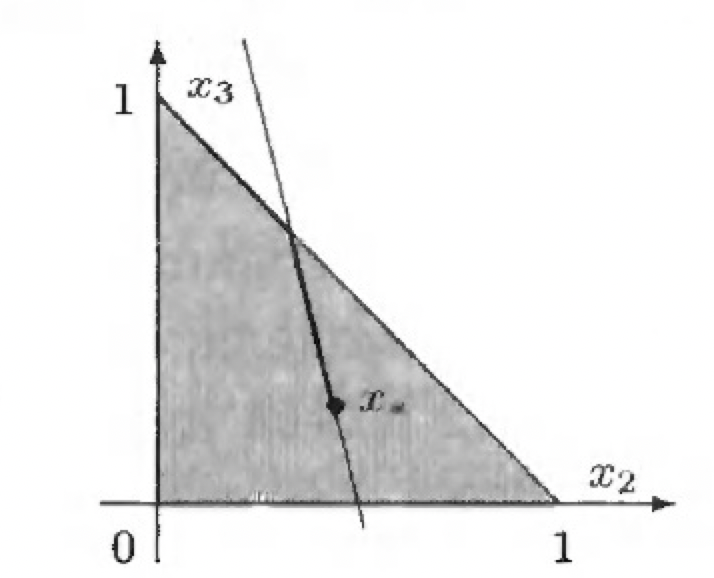
\includegraphics[scale=0.8]{1.png}}
\caption{Пересечение гипотенузы и прямой, прообразом КМР, с уравнением $x_{3} \cong-4.118\left(x_{2}-0.498\right)$}
\end{figure}
\end{enumerate}

\newpage
\section*{5. Список используемой литературы}
\smallskip
\begin{enumerate}
\item[{[1]}] Жуленев С.В. Финансовая математика. Введение в классическую теорию. Ч.2.М.: Издательство Московского Университета, 2012.-432с.
\item[{[2]}] John C. Hull, Options, Futures and Other Derivatives (6th Edition), Publishing house “Williams”, 2008.
\end{enumerate}



\end{document}